\documentclass[12pt]{article}
\usepackage{graphicx}
\usepackage{amsmath}
\usepackage{hyperref}
\usepackage{geometry}
\geometry{a4paper, margin=1in}

\title{Network Traffic Simulation and Modeling in Optical Network-on-Chip (ONoC) Ring Topology}
\author{Daniel Mekonnen}
\date{\today}

\begin{document}

\maketitle

\tableofcontents

\section{Introduction}
\subsection{Overview}
The Optical Network-on-Chip (ONoC) ring topology optimization project aims to enhance the performance of ring-based ONoC networks by addressing critical challenges such as temperature and congestion. This project implements a congestion-aware heuristic algorithm to optimize network traffic and improve overall efficiency.

\subsection{Importance}
Simulation and modeling play a crucial role in understanding and optimizing network traffic in ONoC systems. By simulating various network conditions and configurations, we can identify bottlenecks, evaluate performance, and develop strategies to mitigate congestion and thermal issues.

\subsection{Objectives and Scope}
The primary objective of this mini project is to demonstrate the application of simulation and modeling techniques in optimizing network traffic within ONoC systems. The scope includes developing a simulation model, validating it against real-world data, and conducting experiments to analyze the impact of different parameters on network performance.

\section{Problem Definition}
\subsection{Problem Definition}
Network traffic congestion in ONoC systems can lead to significant performance degradation. The problem involves finding optimal paths for data transmission that minimize congestion and temperature.

\subsection{Real-life Scenario}
ONoC is used in high-performance computing systems where efficient data transmission is critical. Congestion and thermal issues can lead to delays and hardware failures.

\subsection{Assumptions and Constraints}
Key assumptions include a fixed number of nodes and a ring topology. Constraints involve limited computational resources and the need for real-time optimization.

\section{Conceptual Model}
\subsection{Conceptual Model}
The conceptual model represents the ONoC system as a graph with nodes and edges. Nodes represent routers, and edges represent communication links.

\subsection{Diagrams}
\begin{figure}[h]
    \centering
    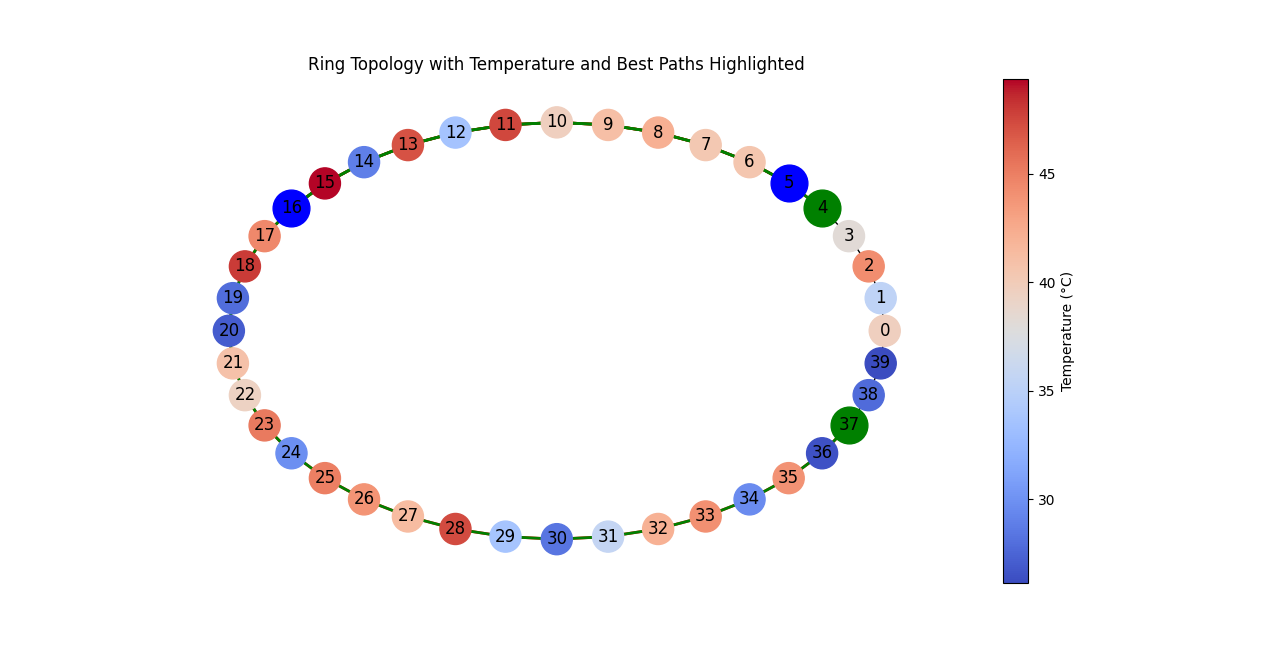
\includegraphics[width=0.8\textwidth]{ring_topology.png}
    \caption{Ring Topology of ONoC}
    \label{fig:ring_topology}
\end{figure}

\subsection{Variables and Parameters}
Variables include node temperature and edge congestion. Parameters include the number of nodes, partition size, and weights for congestion and temperature.

\section{Data Collection and Input Analysis}
\subsection{Data Collection}
Real-world data on network traffic and temperature is collected from high-performance computing systems.

\subsection{Data Sources}
Data sources include network logs and temperature sensors.

\subsection{Input Analysis}
Input data is analyzed to determine distributions and patterns. For example, temperature follows a normal distribution with a mean of 35°C and a standard deviation of 5°C.

\section{Simulation Design}
\subsection{Simulation Technique}
Discrete-event simulation is chosen to model the network traffic.

\subsection{Software Tools}
Python is used as the programming environment, with libraries such as NetworkX, Matplotlib, and Pandas.

\subsection{Simulation Model}
The simulation model is implemented using the existing codebase. It includes functions for creating the ring topology, partitioning nodes, and running the multicast search algorithm.

\section{Model Verification and Validation}
\subsection{Verification}
The simulation model is verified by checking the correctness of the implemented algorithms and ensuring that the simulation runs without errors.

\subsection{Validation}
The model is validated against real-world data to ensure accuracy. For example, simulated temperature and congestion values are compared with actual measurements.

\section{Experimentation}
\subsection{Experiments}
Experiments are designed to test various scenarios, such as high congestion and hotspot scenarios.

\subsection{Simulation Runs}
The simulation is run for different input parameters, such as varying the number of nodes and partition sizes.

\subsection{Output Analysis}
Outputs are recorded and analyzed to evaluate the performance of the TempCon-RingCast and Shortest Path First (SPF) algorithms.

\section{Results and Analysis}
\subsection{Results Presentation}
Simulation results are presented using graphs, tables, and charts.

\subsection{Findings Interpretation}
Findings are interpreted to understand the impact of different parameters on network performance.

\subsection{Insights and Implications}
Insights and implications are discussed, such as the effectiveness of the TempCon-RingCast algorithm in reducing congestion and temperature.

\section{Conclusion}
\subsection{Summary}
The findings of the study are summarized, highlighting the significance of the results.

\subsection{Limitations}
The limitations of the study are reflected upon, such as the assumptions made and the constraints faced.

\subsection{Recommendations}
Recommendations for future work are provided, such as exploring other optimization algorithms and extending the model to other topologies.

\section{Documentation and Appendices}
\subsection{Source Code}
All source code is included in the appendices.

\subsection{Raw Data}
Raw data and additional documentation are provided.

\subsection{User Manual}
A user manual for the simulation is included, explaining how to run the simulation and interpret the results.

\appendix
\section{Source Code}
\subsection{main.py}
\verbatiminput{../src/core/main.py}

\subsection{metrics.py}
\verbatiminput{../src/core/metrics.py}

\subsection{routing.py}
\verbatiminput{../src/core/routing.py}

\subsection{topology.py}
\verbatiminput{../src/core/topology.py}

\subsection{app.py}
\verbatiminput{../src/gui/app.py}

\section{Raw Data}
\subsection{node\_metrics.csv}
\verbatiminput{../results/metrics/node_metrics.csv}

\subsection{partition\_metrics.csv}
\verbatiminput{../results/metrics/partition_metrics.csv}

\subsection{spf\_metrics.csv}
\verbatiminput{../results/metrics/spf_metrics.csv}

\subsection{tempcon\_metrics.csv}
\verbatiminput{../results/metrics/tempcon_metrics.csv}

\end{document}